
\section{DeepPicar Overview}\label{sec:overview}

\begin{figure}[h]
  \centering
  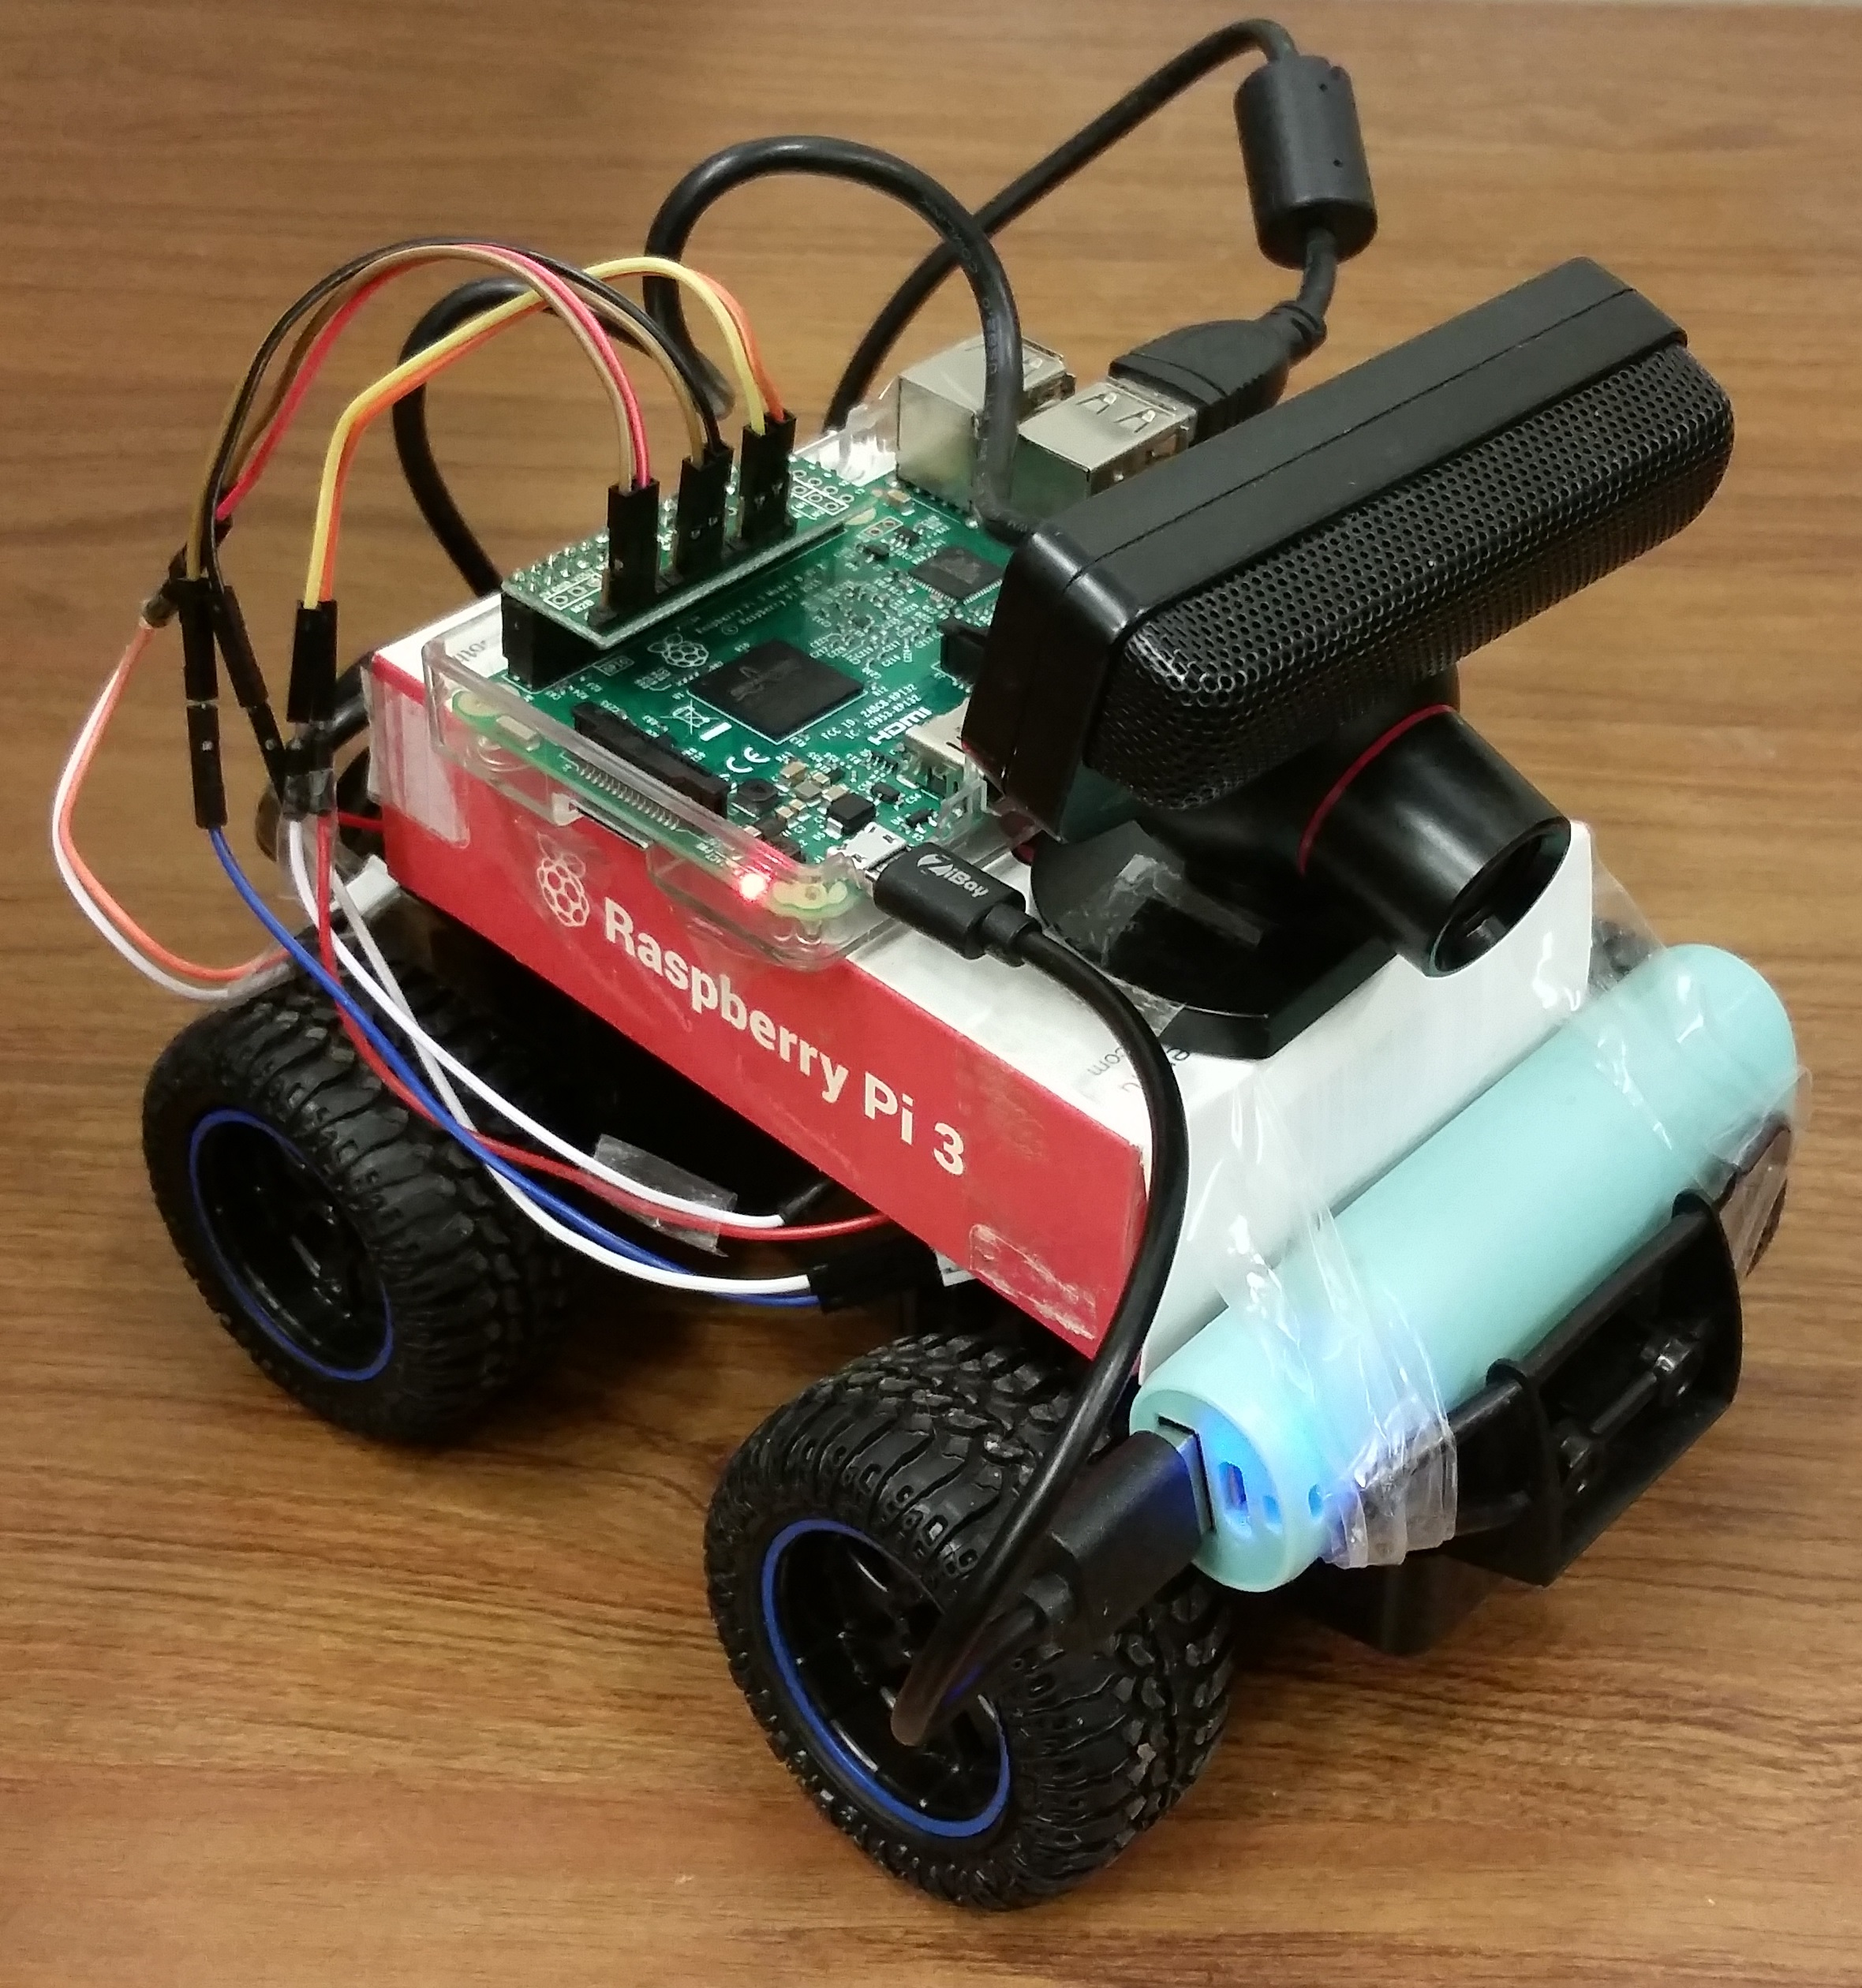
\includegraphics[width=.4\textwidth]{figs/DeepPicar_platform}
  \caption{DeepPicar platform.}
  \label{fig:overview}
\end{figure}

\begin{table}[h]
  \centering
  \begin{tabular}{|c|r|}
    \hline
    Item                    & Cost (\$) \\
    \hline
    Raspberry Pi 3 Model B  & 35 \\
    New Bright 1:24 scale RC car       & 10 \\
    Playstation Eye camera  &  7 \\
    Pololu DRV8835 motor hat&  8 \\
    External battery pack \& misc.   & 10 \\
    \hline
    Total                   & 70 \\
    \hline
  \end{tabular}
  \caption{DeepPicar's bill of materials (BOM)}
  \label{tbl:carbom}
\end{table}


In this section, we provide an overview of our DeepPicar platform.
In developing DeepPicar, one of our primary goals is to faithfully
replicate NVIDIA's DAVE-2 system on a smaller scale using a low cost
multicore platform, the Raspberry Pi 3. Because the Raspberry Pi 3's
computing performance is much lower than that of the DRIVE PX platform
used in DAVE-2, we are interested in if, and how, we can process
computationally expensive neural network operations in
real-time. Specifically, inferencing (forward pass processing)
operations must be completed within each control period
duration---e.g., a WCET of 33.$\overline{\mbox{33}}$ ms for 30Hz control 
frequency---locally on the Pi 3 platform, although training of the 
network (back-propagation for weight updates) can be done offline and 
remotely using a desktop computer.
Figure~\ref{fig:overview} shows the DeepPicar, which is comprised of a
set of inexpensive components: a Raspberry Pi 3 Single Board Computer
(SBC), a Pololu DRV8835 motor driver, a Playstation Eye webcam, a
battery, and a 1:24 scale RC car. Table~\ref{tbl:carbom} shows the
estimated cost of the system.

\begin{figure}[h]
  \centering
  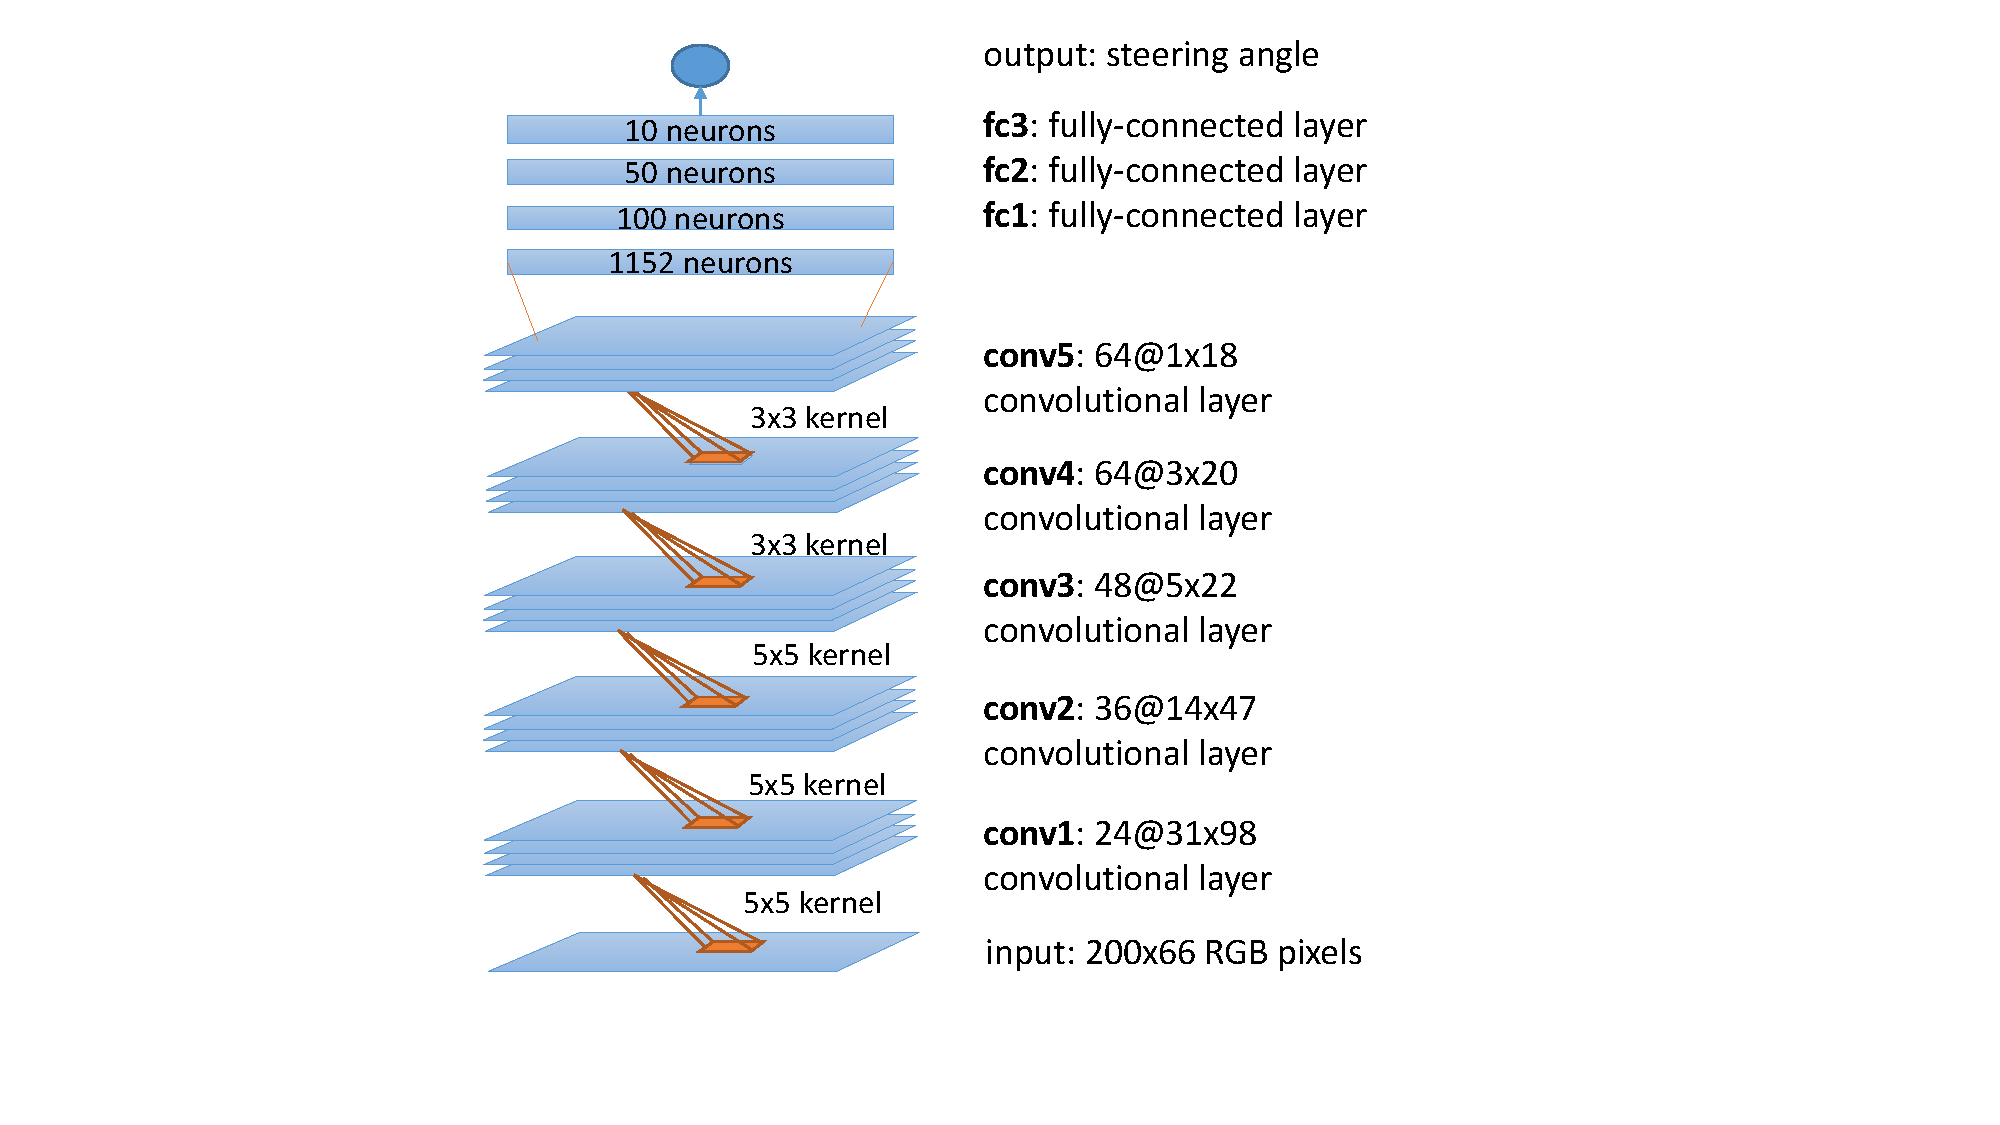
\includegraphics[width=0.4\textwidth]{figs/architecture}
  \caption{DeepPicar's neural network architecture: 9 layers (5
    convolutional, 4 fully-connected layers), 27 million connections,
    250K parameters. The CNN architecture is identical to the one 
	used in NVIDIA's real self-driving car~\cite{Bojarski2016}.}
  \label{fig:architecture}
\end{figure}


For the neural network architecture, we implement
NVIDIA DAVE-2's convolutional neural network (CNN) using a TensorFlow
based CNN model in ~\cite{deeptesla}. Note, however, that the CNN model
in~\cite{deeptesla} was considerably larger than NVIDIA's CNN model as
it contained an additional fully-connected layer of approximately 1.3M
additional parameters. We eliminated the additional layer to
faithfully recreate the NVIDIA's original CNN model.
%% The main difference is that we do not utilize a normalization layer, and 
%% instead initialize the weights using a Xavier initialization. 
As in DAVE-2, the CNN takes a raw color image (200x66 RGB pixels)
as input and produces a single steering angle value as
output. Figure~\ref{fig:architecture} shows the network architecture
used in this paper, which is comprised of 9 layers, 250K parameters,
and about 27 million connections as in NVIDIA DAVE-2's.
%% Note, however,
%% that we did not apply the normalization mentioned
%% in~\cite{Bojarski2016}, as it does not include trainable parameters
%% and its computational demand with respect to the overall CNN
%% processing is minimal.

\begin{figure}[h]
  \centering
  \begin{subfigure}{0.4\textwidth}
    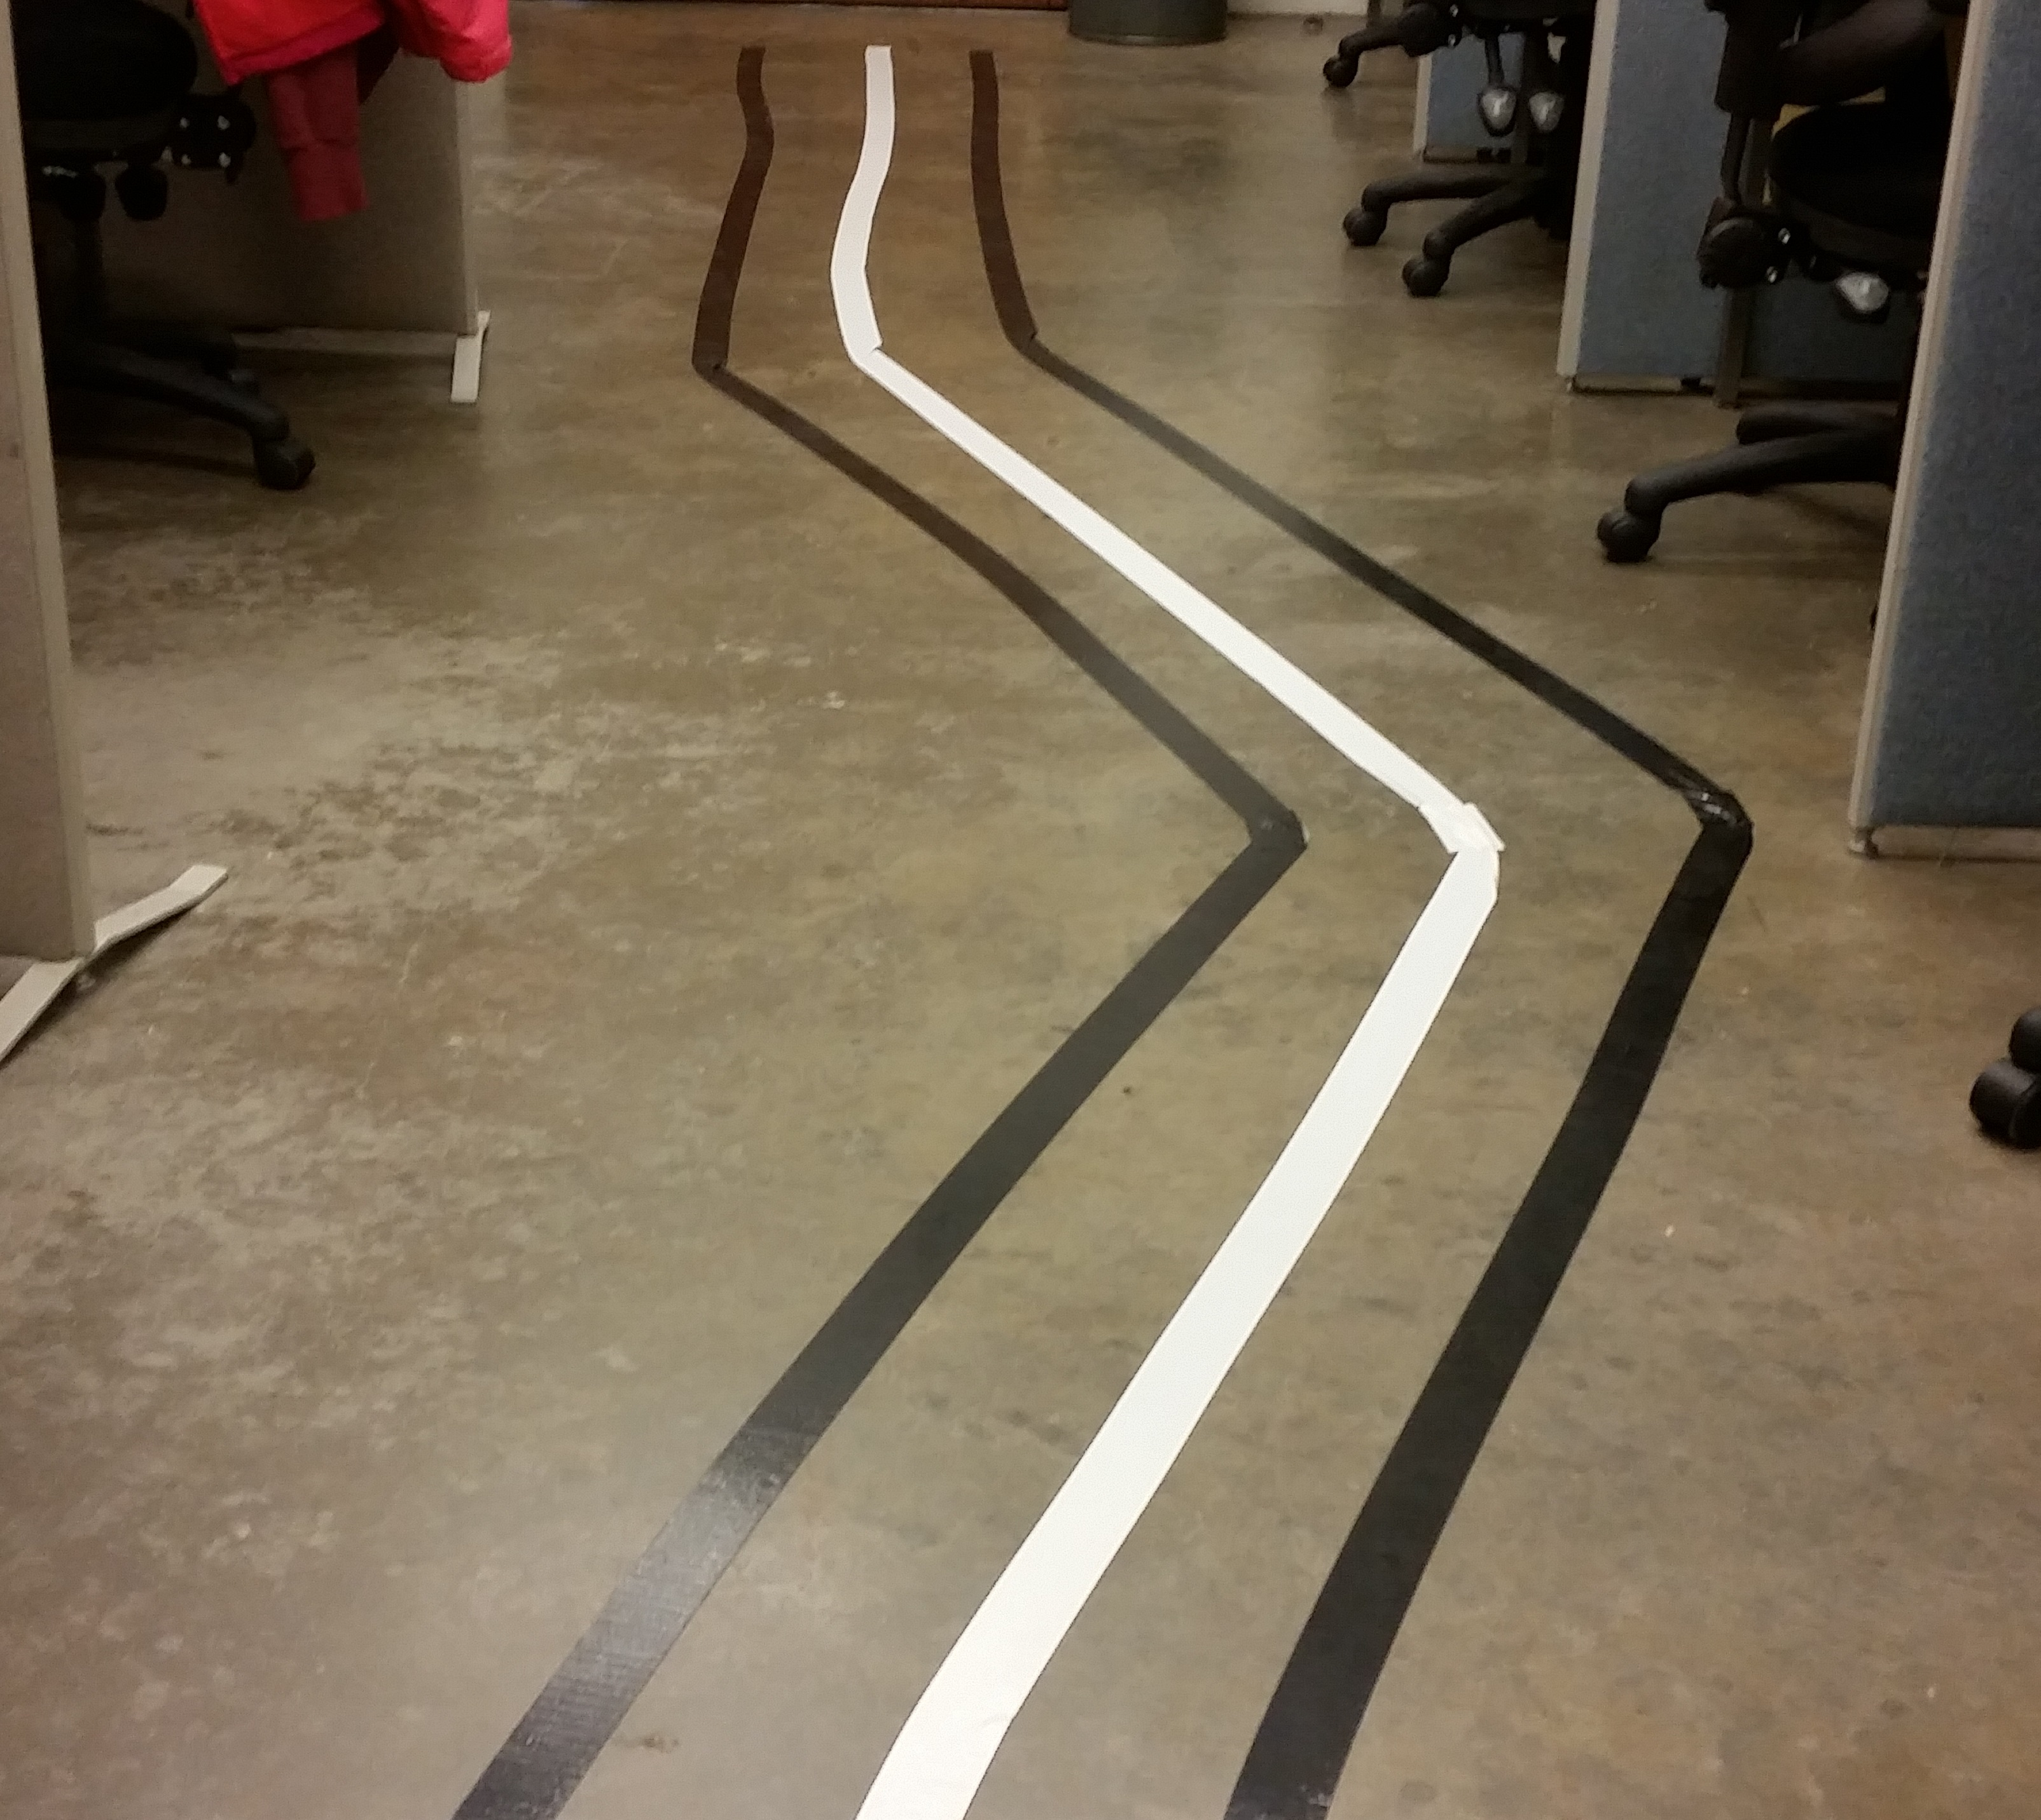
\includegraphics[width=\textwidth]{figs/track_new2}
    \caption{Track 1.}
    \label{fig:track}
  \end{subfigure}
  \hfill
  \begin{subfigure}{0.4\textwidth}
    \includegraphics[width=\textwidth]{figs/track-3}
    \caption{Track 2.}
    \label{fig:track2}
  \end{subfigure}
  \caption{Custom tracks used for training/testing}
  \label{fig:tracks}
\end{figure}

% data collection and training.
To collect the training data, a human pilot manually drives the RC car
on tracks we created (Figure~\ref{fig:tracks}) to record
timestamped videos and contol commands. The stored data is then copied 
to a desktop computer, which is equipped with a NVIDIA Titan Xp GPU, 
where we train the network to accelerate training speed.

%% For comparison, training the network on the Raspbeery Pi 3 takes
%% approximately 4 hours, whereas it takes only about 4 minutes on the
%% desktop computer using the Titan Xp GPU.

\begin{figure}[h]
   \lstset{language=python,
           basicstyle=\ttfamily\small,
           keywordstyle=\color{blue}\ttfamily,
           stringstyle=\color{red}\ttfamily,
           commentstyle=\color{green}\ttfamily
          }  
  \lstinputlisting[language=python]{control.py}
  \caption{Control loop}
  \label{fig:controlloop}
\end{figure}

% inferencing on pi3
Once the network is trained on the desktop computer, the trained model
is copied back to the Raspberry Pi 3. The network is then used
by the car's main controlller, which feeds an image frame from the web
camera as input to the network at each control period. The network
produced steering angle output is then converted into the PWM values
of the car's steering motor. Figure~\ref{fig:controlloop} shows simplified 
pseudo code of the controller's main loop. Among the five steps, the 3rd step, 
network inferencing, is the most computationally intensive and dominates the
execution time.

Note that although the steering angle output of the network ($angle$) is
a continuous real value, the RC car platform we used unfortunately
only supports three discrete angles---left (-30$^{\circ}$), center
(0$^{\circ}$), and right (+30$^{\circ}$)---as control inputs.
Currently, we approximate the network generated real-valued
angle to the closest one of the three angles, which may
introduce inaccuracy in control.
%% In the future, we plan to use a different (more expensive) RC car
%% platform that can precisely control the car's steering angle.

Other issues we observed in training/testing the network, which
can affect the prediction accuracy of the CNN, are camera and actuator
(motor) control latencies. In DeepPicar's
context, the camera latency is from the time the camera
sensor observes the scene to the time the computer actually reads the
digitized image data. This time can be noticable depending on the camera 
used and the performance of the Pi. Higher camera latency could
negatively affect control performance, because the DNN would analyze
stale scenes. Actuator (motor) control latency also can be a
factor, because moving the steering motor to a desired position takes
time. 
In our platform, the combined latency is measured to be around
50 ms. In other words, in the recorded video and control data, a
control action (left, center, right) taken by the CNN appears to be
applied 50 ms later. Considering that camera's framerate is 30Hz
(33.3 ms/frame), this is about two frames after the control action.
%% We experimentally measured the camera
%% latency and found it to be around 50-100 ms.
If this value is too high, control performance may suffer.
Our initial prototype suffered this problem as the observed camera and
control latency was as high as 300 ms, which negatively affected
control performance.
For reference, the latency of human perception is known to be as fast
as 13 ms~\cite{ThomasBurger2015}. 
% https://www.pubnub.com/blog/2015-02-09-how-fast-is-realtime-human-perception-and-technology/

Despite these issues, the trained models were still able to
achieve a reasonable degree of accuracy, successfully navigating
several different tracks we used for training. In our testing, we found 
that the DeepPicar could remain on a fairly challenging track for over 
10 minutes at a moderate speed (50\% throttle), at which point we stopped
the experiment, and more than one minute at a higher speed (75\%
throttle)~\footnote{A collection of self-driving videos can be found
  at: \url{https://photos.app.goo.gl/q40QFieD5iI9yXU42}
  %% \url{https://photos.app.goo.gl/ce93sU7jPk4ywO8u2}
}. Running at
higher speed is inherently more challenging because the CNN controller
has less time to recover from mistakes (bad predictions).  Also, we
find that the prediction accuracy is significantly affected by the
quality of training data as well as various environmental factors such
as lighting conditions. We plan to investigate more systematic ways
to improve the CNN's prediction accuracies.

We would like to stress, however, that
%% the issues related to the
%% CNN's accuracies have no impact on the \emph{computational 
%% aspects of the system}, and that 
our main focus of this study is not in improving the network accuracy
but in closely replicating the DAVE-2's network architecture and
studying its real-time characteristics, which will be presented in the
subsequent section.
